%%%%%%%%%%%%%%%%%%%%%%%%%%%%%%%%%%%%%%%%%%%%%%%%%%%%%%%%%%%%%%%%%%%%
%% I, the copyright holder of this work, release this work into the
%% public domain. This applies worldwide. In some countries this may
%% not be legally possible; if so: I grant anyone the right to use
%% this work for any purpose, without any conditions, unless such
%% conditions are required by law.
%%%%%%%%%%%%%%%%%%%%%%%%%%%%%%%%%%%%%%%%%%%%%%%%%%%%%%%%%%%%%%%%%%%%

\newcommand{\radek}{doc. Mgr. Radek Pel\'anek, Ph.D.}
\newcommand{\umimeCesky}{Um\'ime \v{c}esky}
\newcommand{\ppl}[1]{\textcolor[rgb]{0.6,0.2,1.0}{#1}}
\newcommand{\cviceniB}{``Vyjmenovan\'a slova po B''}

\documentclass[
  printed, %digital, %% This option enables the default options for the
           %% digital version of a document. Replace with `printed`
           %% to enable the default options for the printed version
           %% of a document.
  table,   %% Causes the coloring of tables. Replace with `notable`
           %% to restore plain tables.
  nolof,     %% Prints the List of Figures. Replace with `nolof` to
           %% hide the List of Figures.
  nolot,     %% Prints the List of Tables. Replace with `nolot` to
           %% hide the List of Tables.
  color,
  final,
  nocover
  %% More options are listed in the user guide at
  %% <http://mirrors.ctan.org/macros/latex/contrib/fithesis/guide/mu/fi.pdf>.
]{fithesis3}
%% The following section sets up the locales used in the thesis.
\usepackage[resetfonts]{cmap} %% We need to load the T2A font encoding
\usepackage[T1,T2A]{fontenc}  %% to use the Cyrillic fonts with Russian texts.
\usepackage[
  main=english, %% By using `czech` or `slovak` as the main locale
                %% instead of `english`, you can typeset the thesis
                %% in either Czech or Slovak, respectively.
  english, german, russian, czech, slovak %% The additional keys allow
]{babel}
%% foreign texts to be typeset as follows:
%%
%%   \begin{otherlanguage}{german}  ... \end{otherlanguage}
%%   \begin{otherlanguage}{russian} ... \end{otherlanguage}
%%   \begin{otherlanguage}{czech}   ... \end{otherlanguage}
%%   \begin{otherlanguage}{slovak}  ... \end{otherlanguage}
%%
%% For non-Latin scripts, it may be necessary to load additional
%% fonts:
\usepackage{paratype}
\def\textrussian#1{{\usefont{T2A}{PTSerif-TLF}{m}{rm}#1}}
%%
%% The following section sets up the metadata of the thesis.
\thesissetup{
    date          = 2018/05/28,
    university    = mu,
    faculty       = fi,
    type          = bc,
    author        = Dominik Gmiterko,
    gender        = m,
    advisor       = \radek,
    title         = {Techniques for measuring similarity of educational items},
    TeXtitle      = {Techniques for measuring similarity of educational items},
    keywords      = {adaptive learning, tutoring system, similarity, educational item, similarity measures, explorative analysis, clustering, projections, machine learning, data analysis},
    TeXkeywords   = {adaptive learning, tutoring system, similarity, educational item, similarity measures, explorative analysis, clustering, projections, machine learning, data analysis},
    abstract      = {This work focuses on the measuring of item similarity in tutoring systems utilizing correctness of answers from users. We knew that some unexplained regularities might appear in a similarity of items. In the system \umimeCesky{} they caused separation of items based on their correct answer and level they are assigned into. The core of the work consists of an explorative analysis of possible causes for this regularities. We show that structure of the system can affect item similarities and describe three such factors present in the system. All conclusions were validated using simulations. Our findings are useful for further usage in the analyzed system or replication of similar experiments in other tutoring systems.},
    thanks        = {
    First, I would like to thank my advisor \radek{} for providing me the opportunity to work in the Adaptive Learning group. I want to thank him for giving the right pointers and asking the right questions. I appreciate his expertise and his time he was always willing to find for me.

    My further thanks go other members of Adaptive Learning group, my family, and friends, who were very accommodating of my needs and supported me during my work.

    Finally, I would like to thank all the people who were motivating me to do my best by being smarter than me. Because if you are the smartest person in the room, you are in the wrong room.
    },
    assignment    = task.pdf prohlaseni_autora_skolniho_dila.pdf,
    bib           = thesis.bib,
    style         = fithesis-custom-style
}
\usepackage{makeidx}      %% The `makeidx` package contains
\makeindex                %% helper commands for index typesetting.
%% These additional packages are used within the document:
\usepackage{paralist} %% Compact list environments
\usepackage{amsmath}  %% Mathematics
\usepackage{amsthm}
\usepackage{amsfonts}
\usepackage{hyperref} %% Hyperlinks
\usepackage{markdown} %% Lightweight markup
\usepackage{listings} %% Source code highlighting
\hypersetup{colorlinks, urlcolor=[rgb]{0.6,0.2,1.0}, linkcolor=[rgb]{0.0,0.0,0.0}, citecolor=[rgb]{0.6,0.2,1.0}}
\lstset{
  basicstyle      = \ttfamily,%
  identifierstyle = \color{black},%
  keywordstyle    = \color{blue},%
  keywordstyle    = {[2]\color{cyan}},%
  keywordstyle    = {[3]\color{olive}},%
  stringstyle     = \color{teal},%
  commentstyle    = \itshape\color{magenta}
}
\usepackage{floatrow} %% Putting captions above tables
\floatsetup[table]{capposition=top}
\begin{document}

\hyphenpenalty=9999
\exhyphenpenalty=10000

\hypersetup{linkcolor=[rgb]{0.6,0.2,1.0}}

% --------------------------- %
% Introduction                %
% --------------------------- %

\chapter*{Introduction}
\addcontentsline{toc}{chapter}{Introduction}

% interactive educational systems
% focus on systems with a large number of items

Tutoring systems are computer-based systems designed to teach its users in various domains. They usually consist of a great number of task for users to solve that enables them to provide a personalized experience. To maintain a big pool of items efficiently, we need to be able to decide which items are useful and which are not.

% one possible method, using similarity of items

One possible way how to achieve this is to use similarity of items. The similarity is a basic metric that can be then used in various use-cases, e.g., projections, clustering, and outlier detection. This work discusses different possible similarity measures and differences between them.

% type of work

The basis of the work consists of an explorative analysis of similarity measures and their use cases on a dataset from \umimeCesky{}. We focused especially on using data about user performance from single exercise. We are trying to find the different factors of tutoring system that can affect similarity of items and explain them.

% goal of this work

We want to understand this factors mainly because some of them cause unexpected regularities of items in projections and clusterings. We are using simulations to replicate these regularities and understand them.

% structure of this work

Besides Introduction and Conclusion chapters, this thesis is structured into four main chapters. The first chapter discusses the problem of measuring the similarity of educational items and advantages of using similarity. This chapter also describes previous work and different proposed measures for computing similarity. The second chapter then in detail describes observed problems specific to data we are using. The third chapter gives an overview of many experiments that were concluded. And the last chapter summarizes results and points out practical recommendations.

% --------------------------- %
% Similarity                  %
% --------------------------- %

\chapter{Similarity}

% Intro to chapter, structure

In this chapter, we start with describing specific problem this work is trying to solve. Then we explain what are items (questions) in tutoring systems and how can we compute their similarity. At the beginning of the chapter, we focus on explaining basic terms like tutoring system, item, and similarity that will be used all through the work. Next sections explain why is similarity useful and list its possible usage. The core of the chapter focuses on a description of different kinds of data available about items and possible measures for calculating similarity. In the last portion of this chapter, we discuss previous work in the studied area.

% > Problem

\begin{figure}
    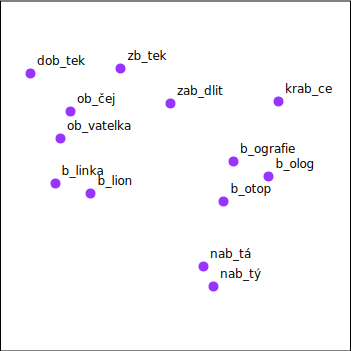
\includegraphics[width=6cm]{img/sample_projection_diagram}
  \caption{Sample projection}
  \label{fig:sample_projection}
\end{figure}

This work focuses on tutoring system \umimeCesky{} that has thousands of items. For management of the items, we want to display them in some way that can be naturally interpreted. Figure~\ref{fig:sample_projection} shows such image. Each dot in the image represents one item, and its proximity to others represents how similar they are. E.g., item ``TODO'' is quite similar to ``TODO'', but it is not similar to ``TODO''.

However, there some unexplained regularities that can appear. They are causing separation of items into clusters which we want to get rid of or at least understand why they are formed.

% > Tutoring systems

\section{Tutoring systems}\label{tutoring-systems}

Tutoring systems are computer systems which purpose is to teach its users (students) some knowledge or skill. These systems do this autonomously to some degree. The degree of automation may vary for each tutoring system.

% Autonomous aspects of tutoring systems

Many different aspects of learning may be implemented into the system, or they may also be left out. The key part of learning is solving educational items. Therefore the most common task which tutoring systems solve is choosing a most beneficial item from the pool of items available for users to solve. The system may adapt to each of the users choosing more challenging and interesting items to users who are more skilled while presenting users who struggle with more basic problems. Choosing correct item is beneficial for maximizing learning aspect of the system~\cite{papouvsek2015impact}. Another aspect which can tutoring systems solve is providing hints and feedback to students. When teachers are interacting with the system, the system can also provide feedback about their students progress and so on.

% > Why is similarity of items useful

\section{Why is similarity of items useful}\label{why-is-similarity-of-items-useful}

% Managing problem pool

In general, there are multiple approaches where we can utilize machine learning techniques to improve tutoring system~\cite{baker2010data}. However, we are focusing only on different usages of similarity of items. This section lists them.

First, most direct, usage is a recommendation of items for a student to solve. We do not want the system to recommend items which are very similar to those that user solved without any problem. However, when user struggled, the system should consider recommending more of the similar problems to strengthen users knowledge.

Another possible usage is generating hints by selecting examples which are similar to the item that is currently solved. Examples are selected from a database of examples. This usage of similarity was previously utilized by Hosseini and Brusilovsky~\cite{hosseini2017study}.

Two previous use cases were using problem similarity to make some choices inside tutoring system automatically. Another approach is to bring humans into the decision-making loop~\cite{baker2016stupid}. This approach provides authors of tutoring system with visualizations that should inform them what changes may be useful. E.g., detecting redundant problems and pointing out where there are not enough similar problems.

One possible way of achieving this is plotting problems to plane and displaying it to the author. This approach still cannot be used for a very large amount of items. However, we choose this approach for our specific dataset as they contain a large number of items, but we do not want to show them all at once. Items are divided into item-sets that are solved independently in the system, and we display only one of them at the time.

Another use-case for similarity is outlier detection. These are items which behave differently from others. This can also be directly visible in projections as such items should lie far away from others or detected from similarity directly.

There is one more usage of similarity that we will not be discussing further. The similarity of items can be utilized for automatic construction of hierarchical categorization. Even when an author already has items categorized, he can compare it to computed categorization to verify that groups are formed correctly and refine them if needed.

% low-level use-cases

Mentioned use cases of similarity are still quite abstract. But there are some standard methods which can be used to achieve them, namely projections, clustering, k-nearest neighbors, and outlier detection that all use similarity. E.g., we can use projections for visualizations, and clustering for construction of categorization.

% > Items

\section{Items}\label{items}

% Why this term

In this work, we use the term ``items'' that may refer to problems, questions, assignments in different systems. Item is a single entry in an educational system which users can answer. Since many aspects of this work are generally applicable, we decided to use this broad term. The complexity of single item in tutoring system can differ greatly. In some tutoring systems, this may refer to simple choice from two options while in other one item is complex tasks which users solves in a matter of minutes.

% Data sources

To further specify the context of our research, we will describe characteristics of items. We can compute similarity in many different ways, but they all have to use data which are available for each item. Therefore we first describe sources of data that can be utilized for measuring the similarity of items.

\begin{itemize}
\item
  \textbf{Item statement} is some specification of the item for a learner to solve, e.g., a natural language description of the task (\ppl{3 + 5 = ?}). Another commonly used format is a grid. Many systems focusing on logic puzzles and programming problems use it.
\item
  \textbf{Item solutions} may provide us with additional information about an item. There will usually be some sample solution (\ppl{8}) provided by the author, and we can also utilize all the solutions from users (\ppl{8, 15, 8, 7\ldots}).
\item
  \textbf{User's performance} consists of information provided indirectly by users. Performance of items may represent user solving times (\ppl{2.8s, 4.0s, 5.1s, 1.0s\ldots}), the correctness of the answers (\ppl{correct, incorrect, correct, incorrect\ldots}), or the number of attempts required.
\end{itemize}

Structure of both item statement and solutions differ considerably based on the context of a tutoring system. However, in general, it is still possible to convert data into some standard form and use one of the common measures despite original format of items.

This description of an item is broad enough to cover most of the tutoring systems. Next chapter discusses more closely tutoring system used for our experiments.

% > Measuring similarity

\section{Measuring similarity}\label{measuring-similarity}

This section explains possible approaches to measuring the similarity of educational items. Following subsections then focuses on specific pipeline we use and comparison of used similarity measures.

Similarity measure quantifies the similarity between two items. Similarity can also be viewed as an inverse of the distance between items, and it can be converted easily as~$1 - \text{item distance}$ or similar.

% what is a similarity, how can we compute it

Items can be converted into vectors of numeric values. This conversion is useful for measuring similarity. For performance data, this is a vector containing correctness or time from all users to given item.

Other properties of items like item statement may also be represented as a vector, e.g., by using a standard technique in natural language processing -- bag-of-words. Method is counting occurrences of each possible word that can appear in item statement. Result is vector of fixed length.

When we have items represented as vectors, we can compare them pairwise to get similarity using some standard similarity measures like Pearson correlation coefficient, Cosine similarity, Sokal measure or Euclidean distance.

% Edit distance

Another possible way to measuring similarity is counting edits which would convert one item to another. This approach is called edit distance, and there are standard ways of computing it for both strings and trees. Edit distance can be then converted into similarity using something like~$1 / (1 + \text{edit distance})$. Therefore we can easily cover another common group of data structures we encounter.

% > > Standard pipeline

\subsection{Standard pipeline}\label{standard-pipeline}

% How is a projection (similarity) computed

To better understand process used to determine similarity of items we have to understand its stage. Following text describes each stage separately. We call this process a standard pipeline, and it is used in most our experiments. When some of the further analysis modify it slightly, it is pointed out in the corresponding section. Whenever we do not specify otherwise, all projections were produced using this default pipeline. There are a few data structures and calculations involved in this process:

\begin{figure}
  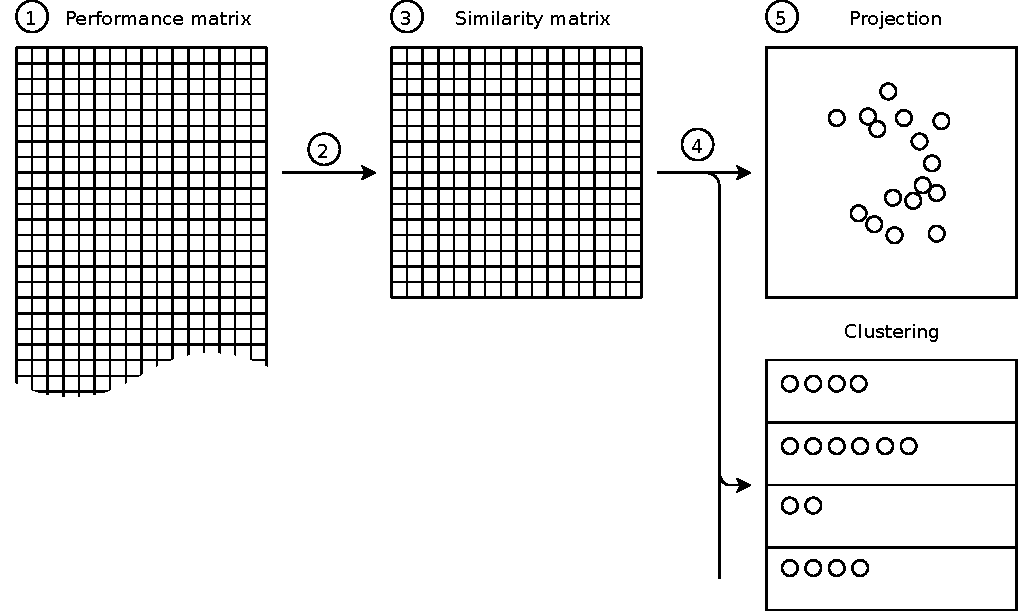
\includegraphics[width=10cm]{img/pipeline_diagram}
  \caption{Diagram showing stages of standard pipeline}
  \label{fig:pipeline_diagram}
\end{figure}

\begin{enumerate}
  \item
    \textbf{Feature matrix} is matrix (items\,$\times$\,features) containing source data. As we said earlier, this could represent any property of items. This matrix consists of one vector for each item, and it may represent item statement, solutions of the item and naturally even users performance.

    The first step we take is converting raw logged information into this matrix. We used correctness of first users answer to a specific item. It will contain value~1~in case of the correct answer and~0~for incorrect. It is worth mentioning that performance matrix is relatively sparse as it is not common for users to solve all the items in the system.

    In our particular case, we call this matrix a \textbf{performance matrix} because it contains information about user performance.

  \item
    \textbf{Measuring similarity} may involve some similarity measure or edit distance. This step is used to compute the similarity between all pairs of items. In other words, we transform feature matrix into similarity matrix. For this stage, we use Pearson correlation coefficient that was selected based on previous work. Values produced by correlation are between $-1$ and~$+1$.

  \item
    \textbf{Similarity matrix} is filled with a pairwise similarity of all items from the feature (performance) matrix. This gives matrix some properties. It is symmetric, and all values at main diagonal are~$1.0$ (because each item is identical with itself).

  \item
    \textbf{Dimensionality reduction} is used to transform similarity matrix into a projection.

    % PCA, (TSNE)

    The similarity matrix is useful for a computer to make a decision based on it directly. However, this matrix still contains way too many values for a human to interpret. As some of our goals are explaining data to authors of the system, we continue with a dimensional reduction to produce a more compact representation of data.

    % PCA over TSNE

    We decided to use Principal component analysis (PCA)~\cite{wold1987principal}, and its first two principal components are then used for 2D visualizations. We choose PCA over other commonly used technique t-SNE (that can produce better-looking results) for one important reason. Results of PCA are deterministic. It produces the same result for same input each time it is run. This is not true for t-SNE~\cite{maaten2008visualizing} that is technique using machine learning and gradient descent for finding some local extreme. Stable results are more suitable for understanding data as there is no variation in results caused by the algorithm. Besides, it is much easier to compare results when altering measure used for computing item similarities.

  \item
    \textbf{Projection} is more compact representation (item\,$\times$\,2) of similarity matrix used for visualizations for end users. There are other possible use-cases of similarity like clustering, or outlier detection but we are focusing on projections.
\end{enumerate}

% Why this pipeline, performance data (not item statement)

We choose this specific pipeline as it can directly utilize data about items performance. In our specific tutoring system performance holds a reasonable amount of information which can be used to calculate item similarity. Other possible choices are using item statement and solutions provided by students. Item statements in our observed exercise consist only of few Czech words with one missing spot. Student solution consists only from a selection between two provided options. Item statement and solutions can be used more effectively in other contexts like programming, mathematics, or physics where item statements are much more complex.

Also, performance is easier to transfer into different tutoring systems because performance is usually available and contrary to item statement performance can be expressed using a standard format (performance matrix).

A similar pipeline was previously used in multiple articles~\cite{pelanek2018programming, kaser2013cluster}. Our choice of a pipeline is also really simple. Therefore it is easy to understand and explain. As it consists only of few steps that can be studied separately and interchanged. It is possible to extend this pipeline for different types of features by adding some pre-processing and post-processing functions~\cite{kaser2013cluster}.

% > > Similarity measures

\subsection{Similarity measures}\label{similarity-measures}

There are many possibilities how to calculate the similarity of two vectors describing the performance of users. As we focus on using performance matrix which contains only two (boolean) values, we can summarize the performance of all users on two items by using just four values using count of encountered answer pairs~\cite{choi2010survey}. Four values are described in Table~\ref{tab:boolean-attributes}. We selected a few similarity measures we are using in this work. They are defined in Table~\ref{tab:boolean-similarity-measures}.

Some of the measures are not using information about correct and incorrect answers symmetrically. For example, Sokal measure uses both $a$ and $d$ interchangeably, but similar measure Jaccard does not. Especially, some metrics ignore value $d$. Therefore we choose to use $a$ as a count of incorrect answers for both items because they are rarer than correct answers.

% Similarity measures definitions

\begin{table}
  \begin{tabular}{ | l | l l | }
      \hline
      \cellcolor[gray]{1.0} & incorrect & correct \\ \hline
      incorrect & $a$ & $b$ \\
      correct & $c$ & $d$ \\ \hline
  \end{tabular}

  \caption{Four parameters of used boolean similarity measures}
  \label{tab:boolean-attributes}
\end{table}

\begin{table}
  \begin{tabular}{ | l | l | }
        \hline
      Pearson & $(ad - bc) / \sqrt{(a+b)(a+c)(b+d)(c+d)}$ \\
      Jaccard & $a / (a+b+c)$                             \\
      Sokal   & $(a+d)/(a+b+c+d)$                         \\
      Cosine  & $a / \sqrt{ (a+b)(a+c) }$                 \\
      \hline
  \end{tabular}
  \caption{Boolean similarity measures}
  \label{tab:boolean-similarity-measures}
\end{table}

% > Previous work

\section{Previous work}\label{previous-work}

Most of the work relevant to our us comes from single article~\cite{pelanek2017measuring}.

They compared few chosen similarity measures to each other. The result was that some of the similarity measures correlate greatly and some do not. It was also determined, based on simulated data, which similarity measures it is best to use for the stability of results. Especially that using Pearson correlation coefficient is a good default choice.

We are also using it for several reasons. The described article showed that it has good enough results in producing distinct clusters on performance data. Another reason is that Pearson correlation is easy to use as many computational environments already contain fast implementation.

The article also showed that using the ``second level of similarity'' improves the stability of results further. However, we choose not to use it as using more straightforward measure is beneficial when explaining results and this factor is important to our work.

% --------------------------- %
% Used datasets               %
% --------------------------- %

\chapter{Used dataset}\label{used-dataset}

The first half of this chapter focuses on used sources of data. It describes both simulated data and dataset from the actual system. We outline structure of tutoring system and focus on exercises and its objects that are useful for our work. Another section includes basic statistics about data from \umimeCesky{}. End of the chapter provides an example of the simple projection and description what properties should useful projection have. The last section describes problems we are trying to solve and specific questions this work tries to answer.

% types of data (real, simulated), why, real, simulated

In our analysis, we use both real data from the educational system and simulated data. Reason for this is that real-world data are useful for concluding any practical results. However, evaluation of this data is often complicated as we do not know the truth about many of its aspects. That is why we also use simulated data for validating some of our conclusions.

% > Simulated data

\section{Simulated data}\label{simulated-data}

When simulating data, we are trying to generate results which are similar to real tutoring system. However, we use much simpler model. Similar models were previously used in multiple studies~\cite{piech2015deep, pelanek2017measuring}.

The result of the simulation consists mainly of performance matrix with items as columns and users as its rows. First, we have to generate items. For each item, we choose its difficulty and skill required to solve this item. The difficulty of item is value drawn from normal distribution $\mathcal{N}(0,\,1)$.

After that, we continued with the construction of users. We generate skills for all the users. They are random values from normal distribution $\mathcal{N}(0,\,1)$ and are stored in a user\,$\times$\,skills matrix.

Next, we simulate each user answering to each item. The user answers correctly with probability given by a logistic function of the difference of item difficulty $d$ and user skill $s$. User skill is one of the his skills that corresponds to the skill required for given item.

\begin{gather*}
\sigma(x) = \frac{1}{1 + e^-1x} \\
\text{then}\\
P(\text{correct}|s, d) = \sigma(s - d)
\end{gather*}

We will talk more in depth about how we generated simulated data in next chapter when describing how we used them specifically. In all experiments using simulated data, we altered this basic simulation in some way to achieve results corresponding to some attribute of real data.

% > Umime cesky

\section{\umimeCesky{}}\label{umime-cesky}

% Czech grammar, ``fill-in-the-blank'' with two choices

\href{https://umimecesky.cz/}{Umíme česky} is a system for practice of Czech grammar. This section describes the tutoring system, exercise used in our analysis and lists basic statistics about dataset size.

The system contains multiple exercise types, but in our analysis, we use only one exercise type. It is simple ``fill-in-the-blank'' with two possible answers. A user is asked to choose one of them. This is shown in Figure~\ref{fig:umimecesky_doplnovacka}. After answering user receives feedback whether the answer was correct or not. Answers are always displayed in alphabetical order, so their position does not change when solving different items.

Although we focused only on ``fill-in-the-blank'' exercise, it can still be used to train various concepts of Czech grammar. The over 6000 questions in this exercise. They are divided into item-sets. Each item-set consists of items practicing a different aspect of language, e.g., \cviceniB{} or ``Velká písmena: státy, oblasti''. This item-sets are arranged into hierarchical categorization as seen in the user interface. Since our analysis works only with item-sets separately this categorization into different aspects is not important to us. After the user chooses some item-set the questions are selected randomly, so we consider that the items in each item-set are solved uniformly. Therefore we can compare them without any bias of user selection.

Items in item-sets are divided into levels. Higher levels are intended to be solved by more experienced users as they contain more difficult questions. In general, there are three difficulty levels, but not all item-sets have all three of them. Some easy item-sets include only first level. On another hand, there are item-sets which have all three levels or only higher levels.

\begin{figure}
  
\includegraphics[width=7cm]{img/umimecesky_doplnovacka}
  \caption{Sample question from ``fill-in-the-blank'' exercise in \umimeCesky{}}
  \label{fig:umimecesky_doplnovacka}
\end{figure}

% information about items: question, correctness and time

The used dataset contains multiple sources of information about items. We have item statement which consists of a question with one missing spot (\ppl{``živob\_tí''}) and two possible answers to fill in there (\ppl{``i''} and \ppl{``y''}). There are also available all the answers from users. The last two sources of available information are correctness of user answers and their response time.

However, it is not possible to use response time directly. We need to normalize it in some clever way as raw response time is greatly affected by both lengths of questions and users reading speed. Also, it is a good idea to use a logarithm of time instead of time itself~\cite{niznan2014using}. Only then it would be useful to use data about response times.

% Why this system

We choose this tutoring system because, as we explained before, we are focusing on problems which are most important for systems with a large number of items. Also provided dataset has a large number of users and answers which is great for the stability of results.

% > > Basic statistics

\subsection{Basic statistics}\label{basic-statistics}

\begin{table}
  \begin{tabular}{|l|r r r|}
    \hline
    \cellcolor[gray]{1.0} & Items & Users & Answers \\
    \hline
    Whole exercise & 6\,037 & 46\,128 & 10\,421\,521 \\
    \cviceniB{} & 273 & 14\,207 & 1\,216\,403 \\
    \hline
  \end{tabular}
  \caption{Basic statistics of dataset}
  \label{tab:basic-statistics}
\end{table}

This section provides some basic statistics about the size of dataset and users of the system. Table~\ref{tab:basic-statistics} shows number of items, users and answers. Statistics describe both dataset globally and one selected item-set \cviceniB{} that is most commonly used for our analysis. This item-set has most answers from users. Therefore, it is ideal for analysis because results are more stable. We mostly used this item-set, but we also confirmed observed behavior on other item-sets.

% Users using the system

A primary group of users using \umimeCesky{} are children studying at primary and secondary school. Users can have individual accounts, but the system also allows teachers to create a virtual class and assign students to it. A teacher is then able to select some exercises and give them to students to solve until some deadline. Each week about 200 classes visit the system.

% > Visible properties of projections

\section{Visible properties of projections}\label{visible-properties-of-projections}

\begin{figure}
    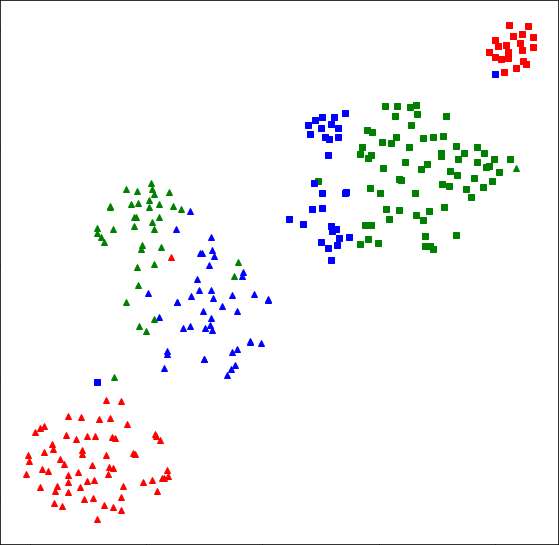
\includegraphics[width=\textwidth]{img/common_projection}
  \caption{Basic projection of item-set \cviceniB{}. Three used colors distinguish levels and markers correct answers of items. The highlighted group (items inside the circle) contains words starting with prefix ``bio'' that are correctly considered similar and appear close to each other. On the other hand, two connected items should be considered similar, but they are not because they are in different levels.}
  \label{fig:common_projection}
\end{figure}

% why is projection useful

Projections come in handy when it is hard to understand data directly because there is way too much of them. And this is our case as we focus on systems which consist of thousands of solvable items and even more users. Projections are results of dimensionality reduction techniques. They project many-dimensional data into fewer (usually two) thoughtfully chosen dimensions to simplify them.

% similarity and projection

In general, we want projection which puts similar items together. This property can be achieved in many different ways. The following section explains choices we made when selecting a source of data, a method of processing them before applying dimensionality reduction, and dimensionality reduction technique itself.

% Visible properties of a projection

Figure~\ref{fig:common_projection} shows how can resulting projection look like. This particular projection shows 273 items (single item-set). Each item is represented as one dot in the image, and its proximity to others represents how similar they are. There are no labels on plot axis as dimensions of projection cannot be named explicitly only the proximity of items is preserved.

% Similar words near each other

As projections are meant to be used for managing item pool, this puts some constraints on how ideal projection should look like.

We want similar items to end as close to each other as possible. In particular, when using performance as a source of data, we can interpret this as items which require same skills should be projected near each other. For example, when we look at item-set \cviceniB{} (Figure~\ref{fig:common_projection}) there is encircled group of words starting with common prefix ``bio''. It is correct that they are close to each other as they are indeed similar because they are based on a single word. But remember, there is no information about item statement presented to the similarity measure.

% > Regularities

\section{Regularities}\label{regularities}

% This causes similar words to end-up far away one from another

Projections of item-sets from system \umimeCesky{} (Figure~\ref{fig:common_projection}) all display some regularities. Items depicted with same colors and items using same markers form clusters. This section talks about formed clusters in projection and why it is a problem.

% > > Level regularity

\subsection{Level regularity}\label{regularities-level-regularity}

% Description of problem, three clusters based on three levels of questions difficulty

Figure~\ref{fig:common_projection} contains items of three different colors. Item-sets in system \umimeCesky{} are divided into multiple levels of difficulty. For this particular item-set, there are three difficulty levels. The first level is depicted using purple (with 110 items), second orange (with 86 items), and third green (with 77 items). There is a visible pattern in our data. Items from the same level are forming clusters.

As we mentioned before, only data about user performance (correctness of answers) are used when composing projections. And there is not a direct reason for this clusters of same levels to form as no information about belonging to a particular level is presented to the algorithm.

% why is this unsuitable, example of similar words far away one from another

This phenomenon is not suitable for analysis of item similarity as it can cause misleading results about similarity. One particular example is when similar words are displayed far away from one another just because they belong to different levels. Such example is pair of words ``bič'' and ``bičík'' in item-set \cviceniB{}. They are connected by a line in the Figure~\ref{fig:common_projection}.

% > > Answers regularity

\subsection{Answers regularity}\label{answers-regularity}

Another property of items in Figure~\ref{fig:common_projection} is depicted by a marker used. One type of marker (rectangle) shows items with correct answer ``i'' and another marker (triangle) shows items with correct answer ``y''. Again, there is no direct information about this presented to measure of similarity, but such clusters form despite it. So it is useful to explore why is this behavior present at all.

% > > Research questions

\subsection{Specific questions}\label{specific-questions}

There are several main questions we are trying to address:

\begin{itemize}
 \item Which high-level factor in data can cause these regularities?
 \item Is there multiple factors causing these regularities?
 \item Can we explain them sufficiently?
 \item Are we able to replicate this factors on simulated data?
\end{itemize}

% general to be continued text

Following two chapters are focusing on this questions. First, we describe concluded experiments and then summarize conclusions.

% --------------------------- %
% Evaluation                  %
% --------------------------- %

\chapter{Evaluation}\label{evaluation}

The chapter is describing several experiments we concluded to find factors that can affect resulting projections produced from real-world data. We are focusing on higher level factors that can cause a formation of clusters in projection. On a low level, it is apparent that items which have similar answers will be similar (close to each other) in projection.

% > Basic

\section{Basic}\label{evaluation-basic}

The first section is focusing on experiments which determine a range of this behavior. We ask whether clusters of same answers or levels are still present when altering parameters of pipeline used to calculate projection.

% > > First and last users answer

\subsection{First and last users answer}\label{first-and-last-users-answer}

% Why bother about this

Our performance matrix contains only one value for each item-user pair. But users can answer to the item multiple times. This raises a question about which of user answers to use.

% What we used in performance matrix

We tried using both first users answer and last in performance matrix. However, there is no visible difference in results. This is clear when we compare first and last answers of users. There is only 5\% difference between them. So at least with a large number of items in the system it does not matter which one is chosen as only a few items are answered multiple times.

% > > Level of regularity on different item-sets

\subsection{Level of regularity on different item-sets}\label{level-of-regularity-on-different-item-sets}

When introducing the problem of unneeded clusters in section~\ref{regularities} we showed that one particular item-set shows this behavior. However, we we did not show whether this is true for all the item-sets. We decided it may be useful to quantify how recognizable are this clusters on all item-sets.

% Quantification of level-answer clustering

Quantification of the regularity of clusters in the projections is executed using k-means and adjusted Rand index. We use the k-means clustering algorithm~\cite{hartigan1979algorithm} to find \textit{levels\,$\cdot$\,correct answers} clusters in data about item similarity. Level of regularity is then determined using adjusted Rand index~\cite{santos2009use}. We compare extracted clustering with the original one (clusters created as a combination of item level and correct answer). Value~1.0 represents that k-means was able to divide all items into same clusters as original classification. On the other hand, lover values show that it is hard to divide items correctly and there are no distinct clusters. This process is repeated multiple times to account for random initialization of k-means algorithm.

\begin{figure}
  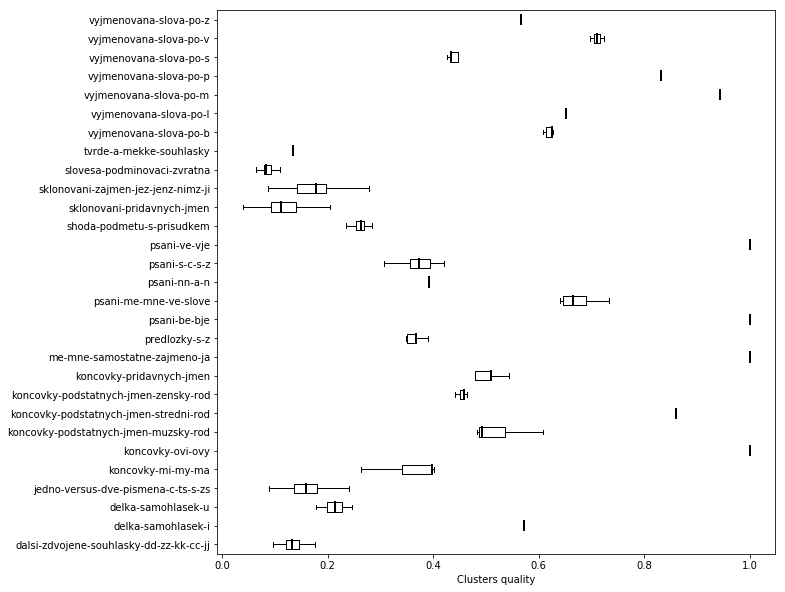
\includegraphics[width=\textwidth]{img/clustering_quality}
  \caption{Evaluation of cluster quality on different item-sets}
  \label{fig:clustering_quality}
\end{figure}

Figure~\ref{fig:clustering_quality} describes level of regularity of different item-sets. Results show that many item-sets have distinct clusters of different levels and answers. However, there are some item-sets with an obscure structure of similarity. This mostly occurs when item-set have a large number of different answers. It is worth mentioning that even when some item-sets do not have a high score when comparing extracted clusters to actual but results are stable across runs of k-means. Which also suggests that projections have nicely visible clusters but items are not divided (only) by levels and answers.

% Conclusion

We can conclude that regularities are present in some form in all item-sets.

% > > Similarity measures

\subsection{Similarity measures}\label{evaluation-similarity-measures}

Another question is whether using Pearson correlation coefficient is not cause of some of the regularities. Therefore, we tried exchanging measure used for computing similarity of items to verify that previous results are not specific to a single measure. We evaluated all four previously chosen measures.

% preserving of clusters

\begin{figure}
  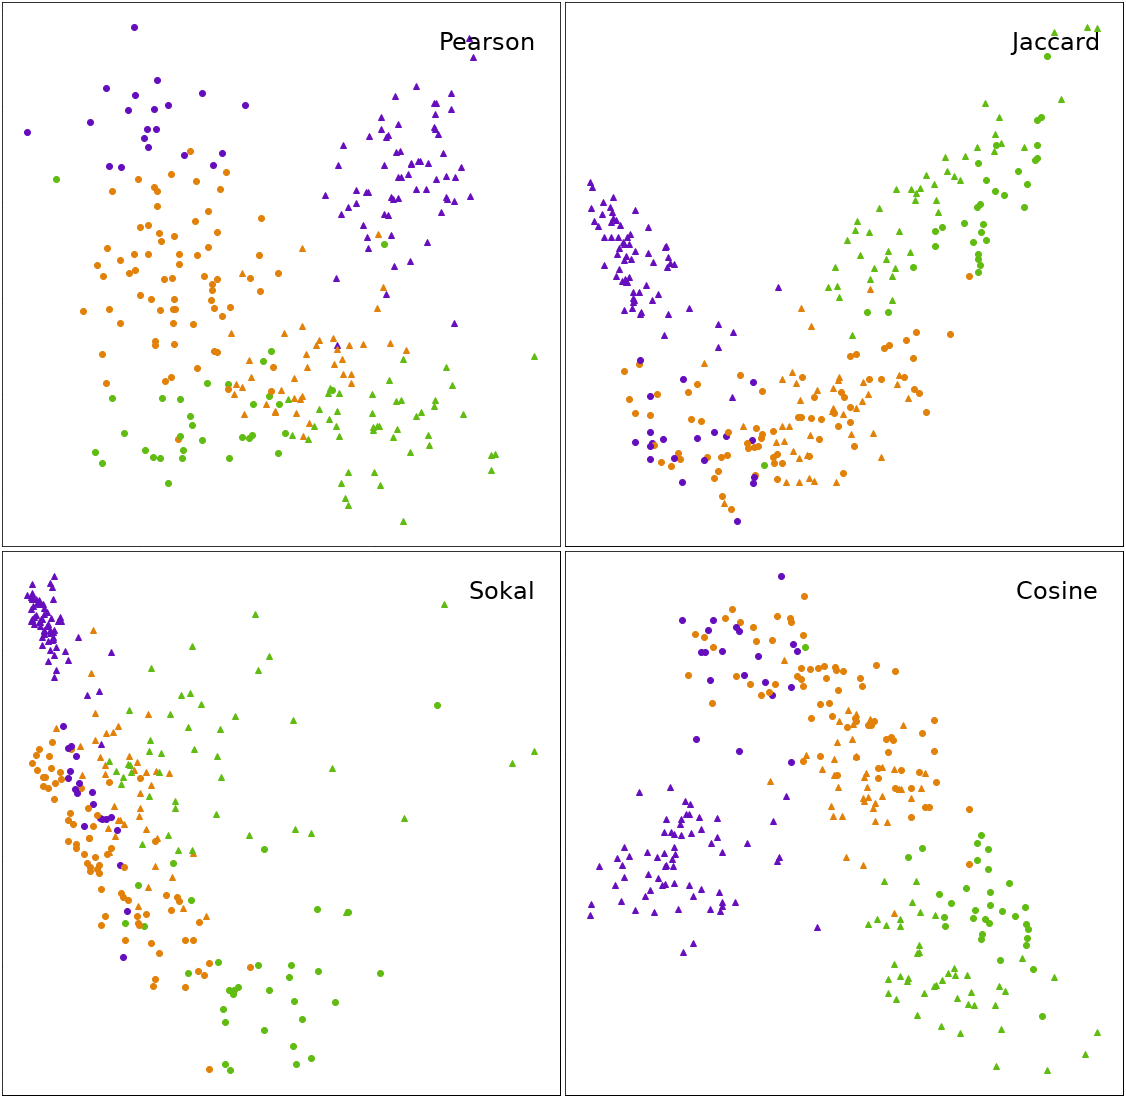
\includegraphics[height=10cm]{img/measures}
  \caption{Comparison of four similarity measures projected by PCA using the same item-set}
  \label{fig:measures}
\end{figure}

Figure~\ref{fig:measures} shows four different similarity measures used on same data. Resulting projections are different. However, they all preserve information which is causing items from the same level and same answer to form clusters. Used colors represent different levels and markers are used to distinguish different answers.

% Visible comparison

\begin{itemize}
\item
  \textbf{Pearson} is the most commonly used measure.

\item
  \textbf{Jaccard} differs visibly from other measures. Resulting projection still shows same clusters of levels and items are split based on a correct answer, but the similarity of the items does not correlate with correlation-based measures like Pearson.

\item
  \textbf{Sokal} shows best that different similarity measures can highlight different aspects of item performance. The similarity of items depends heavily on the performance of items when using Sokal. (Where performance of item is the number of correct answers divided by all answers.) Items with higher performance are much more similar than items with lower performance. This property is causing a packed cluster of items from a first level (easy) and a spread out cluster of items from third level (harder).

\item
  \textbf{Cosine} similarity produces projection very similar to Jaccard only mirrored vertically.
\end{itemize}

We can conclude that clusters are present despite used similarity measure.

% > Answers regularity

\section{Answers regularity}\label{evaulation-answers-regularity}

This section describes in detail some of our experiments we concluded that relate to separation of items into clusters of same correct answers. We describe four experiments in total. They brought us to finding one more regularity, and in the end explaining separation items by their correct answer.

% > > Total similarity of items

\subsection{Total similarity of items}\label{total-similarity-of-items}

When exploring data, it may be useful to detect outliers. One possible way of how to detect an outlier is looking at the sum of its similarities or distances to other $k$ nearest neighbors. This was done for example by Zhang and Wang~\cite{zhang2006detecting}. In particular, this means that an item with a low sum of similarities to other items may be an outlier. At this point, we encountered another regularity in data. It was detected that items with some correct answer might have greater similarity than other answers. This regularity could cause problems with using such outlier detection as items having some correct answers have a higher probability to be selected as an outlier, and it is not true.

For this purpose, we define another property of items. The total similarity is a sum of one items vector of similarities (one column of similarity matrix) to other items. This property is normalized to range 0.0-1.0 and tells us how much is item similar to other items. Histograms of two possible answers of item-set \cviceniB{} is displayed on Figure~\ref{fig:histogram_i_y}. It is visible that items with answer ``i'' has higher total similarities that items with answer ``y''.

\begin{figure}
  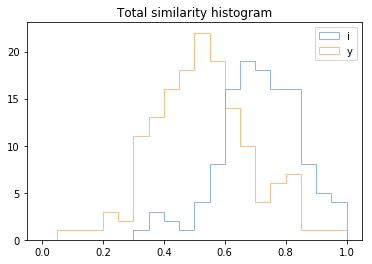
\includegraphics[width=10cm]{img/histogram_i_y}
  \caption{Histograms of total similarities of items divided by correct answer on one item-set}
  \label{fig:histogram_i_y}
\end{figure}

% total similarity histograms divided by answer

% other item-sets

This is not specific to only one item-set (displayed in Figure~\ref{fig:histogram_i_y}) almost all item-sets display similar pattern. Although for some item-sets, it is more distinct than for others. Sets consisting of items with many possible answers does not behave this way. But that is to be expected.

We picked few item-sets which have very distinct clusters of answers and looked whether the answer with higher similarity is located on the left or the right in the user interface. (User interface was shown in second chapter~\ref{fig:umimecesky_doplnovacka}.) We found that preferred answer could be located on both left and right button. In particular, in concept \cviceniB{} that have possible answers ``i'' (left) and ``y'' (right) the preferred one is the left answer. But for concept ``Koncovky přídavných jmen'' that has the same possible answers is preferred one ``y'' on the right.

This experiment told us only that there is some underlying difference between items with different correct answers but did not tell us what.

% > > Performance matrix

\subsection{Performance matrix}\label{performance-matrix}

Performance matrix shows answers from users to items. Each column in Figure~\ref{fig:performance_matrix} depicts answers to one item. Each row corresponds to one user and colors represent correctness of answer (green is correct, red incorrect) or missing answer (gray). Items (columns) in the matrix are sorted that all items with correct answer ``i'' are on the left and items with another possible correct answer ``y'' are on the right.

\begin{figure}
  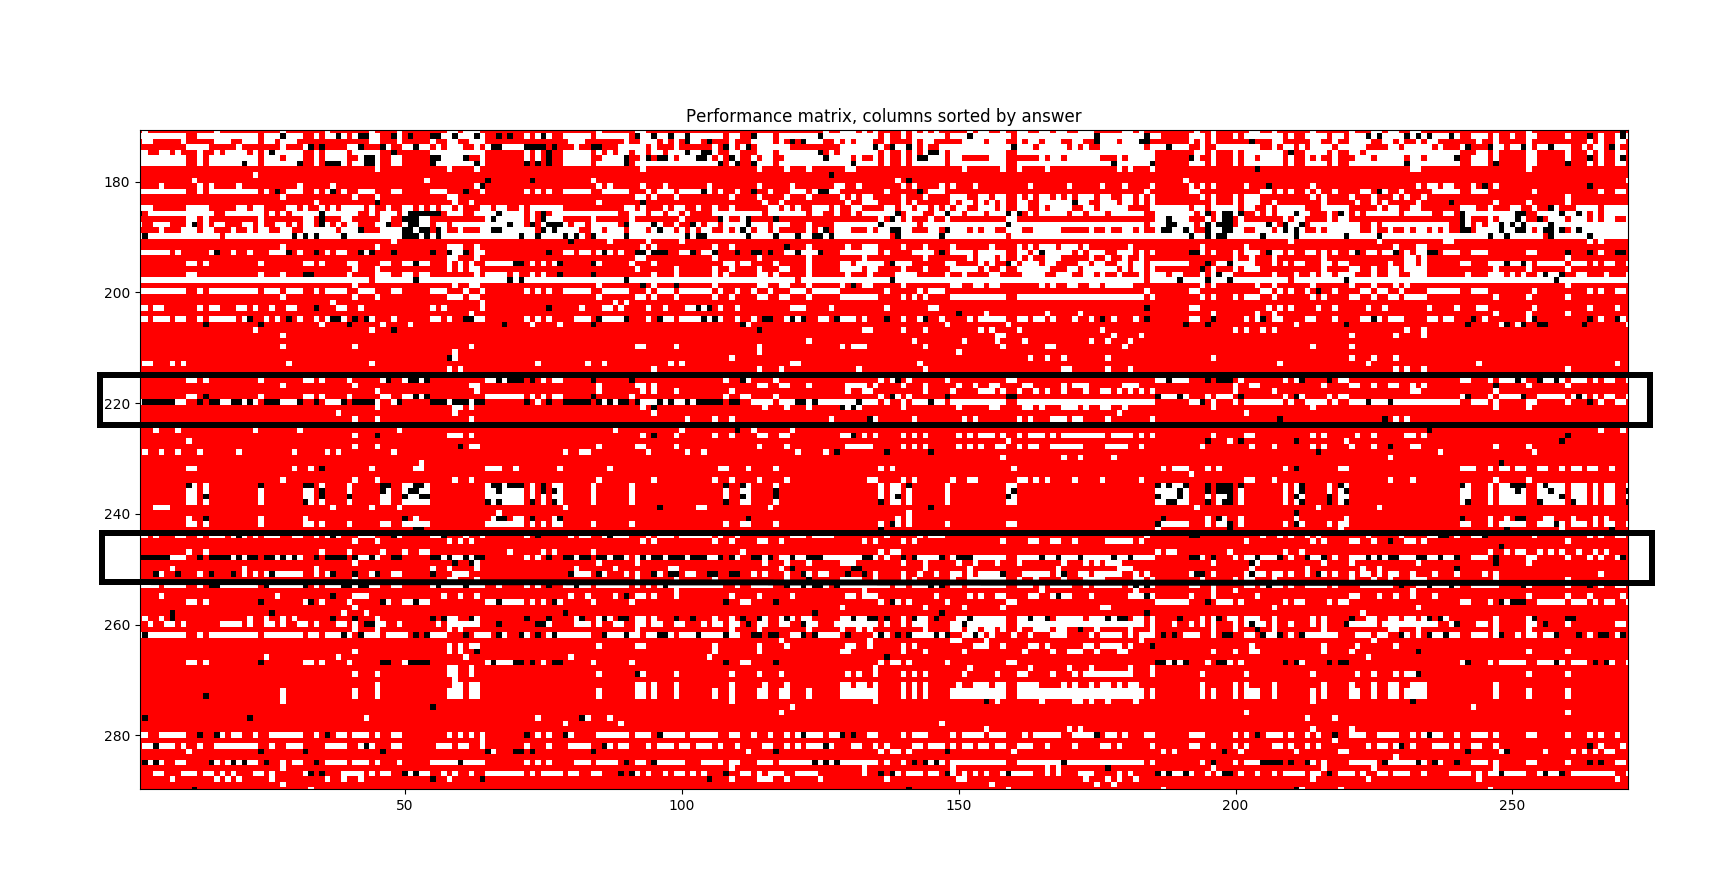
\includegraphics[width=10cm]{img/performance_matrix}
  \caption{Part of performance matrix with highlighted row contains uneven answers from single user (green - correct, red - incorrect, gray - missing)}
  \label{fig:performance_matrix}
\end{figure}

After exploring performance matrix some more, we can see that there are users who have much higher performance on items with one answer than another. This can be seen in highlighted row of Figure~\ref{fig:performance_matrix}. He answered almost all items with one answer (right) correctly and items with another answer (left) incorrectly. There are even users who almost always use one of the answers.

% > > Default answer

\subsection{Default answer}\label{default-answer}

We guessed that there are users who prefer using one answer by default when they do not know the answer. Firstly we wanted to determine whether preferring one answer over another can affect projection and create clusters of different answers.

We used simulation for this. Simulation was slightly refined over basic simulation described in second chapter~\ref{simulated-data}. There are a few differences over basic simulation. For each item, we also choose a correct answer. We use it to offset logistic function higher or lower to simulate higher chance of succeeding when solving items which correct answer is the users preferred one. In this experiment, we used offset 0.2 which corresponds to 20\% higher chance to answer correctly one answer and 20\% lower on items with another answer. Also, there are no missing values in performance matrix as simulated users answer to all items.

This specific simulation is using two uncorrelated skills and two answers. They are distributed in a way that there is the same amount of each combination (1/4 of items). We included two skills in this simulation to better illustrate conditions in real data.

\begin{figure}
  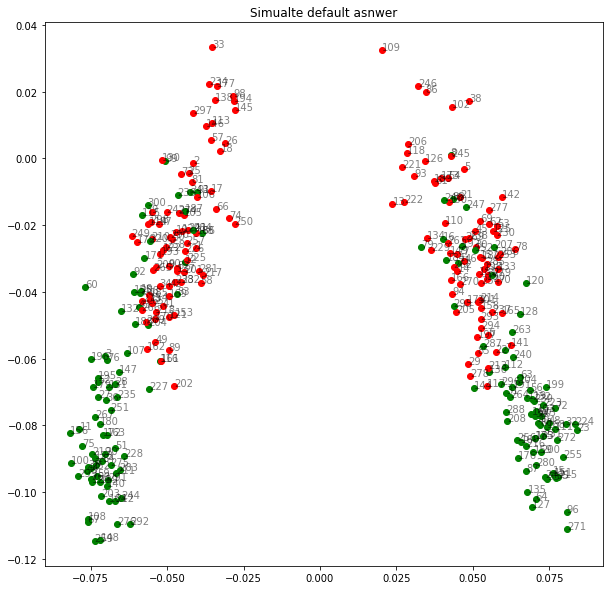
\includegraphics[height=8cm]{img/simulated_default}
  \caption{Projection of simulated data using default answers when user does not know how to answer}
  \label{fig:simulated_default}
\end{figure}

When we look at resulting projection~\ref{fig:simulated_default} of simulated performance data we can see that it has same properties as our real data. There are clusters (in this case caused by uncorrelated skills) that have items separated by the correct answer (represented by different colors).

We conclude that users preferring one answer over another can cause separation of items by correct answer in projection.

% > > User answer performance

\subsection{User answer performance}\label{user-answer-performance}

% how to detect this in real data

The previous simulation showed that preferred answer could cause separation of items. Now we have to show that users like this exist in our real dataset.

We observed before that whole dataset uses both answers approximately the same, but for a single user, this may not be true. In this experiment, we want to quantify whether each user prefers some answer or not. For this, we used a difference of user answer performances.

User answer performance is calculated as a ratio of items which user answered correctly to all items when looking only at items with a particular correct answer. We calculate this value for each possible correct answer and each user. Then we combine this set of user answer performances for each user to one value using their difference. This metric gives us single value representing whether the user uses some answer by default. Value ranges from 0.0 that represents no preferred answer at all to 1.0 which is largest possible preference.

\begin{figure}
  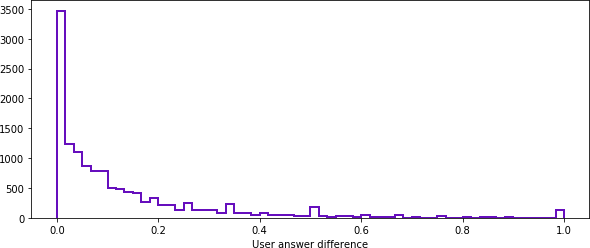
\includegraphics[width=10cm]{img/uneven_answers_hist}
  \caption{Histogram of user answer performance difference}
  \label{fig:uneven_answers_hist}
\end{figure}

Figure~\ref{fig:uneven_answers_hist} shows histogram of user answer differences on one item-set. There are few visible groups of users. The largest group have uniform performance on all answers (represented by values close to 0.0). On the other end of the spectrum are users who use only one answer (values close to 1.0). Users in the middle of spectrum probably prefer one of the answers but use both. It is visible that there is quite a large amount of users with a small preference for one of the answers. (It does not matter which one.)

% metric reasoning

We choose to use a difference of performance instead of how much user uses each answer because we do not have to normalize it in any way. If we choose to use usage of answers we have to compare this to correct ratio as it is not guaranteed that item-set contains the same amount of items for all correct answers. Using difference of performance resolves this for us.

% similar items from different levels are little closer to each other

\begin{figure}
  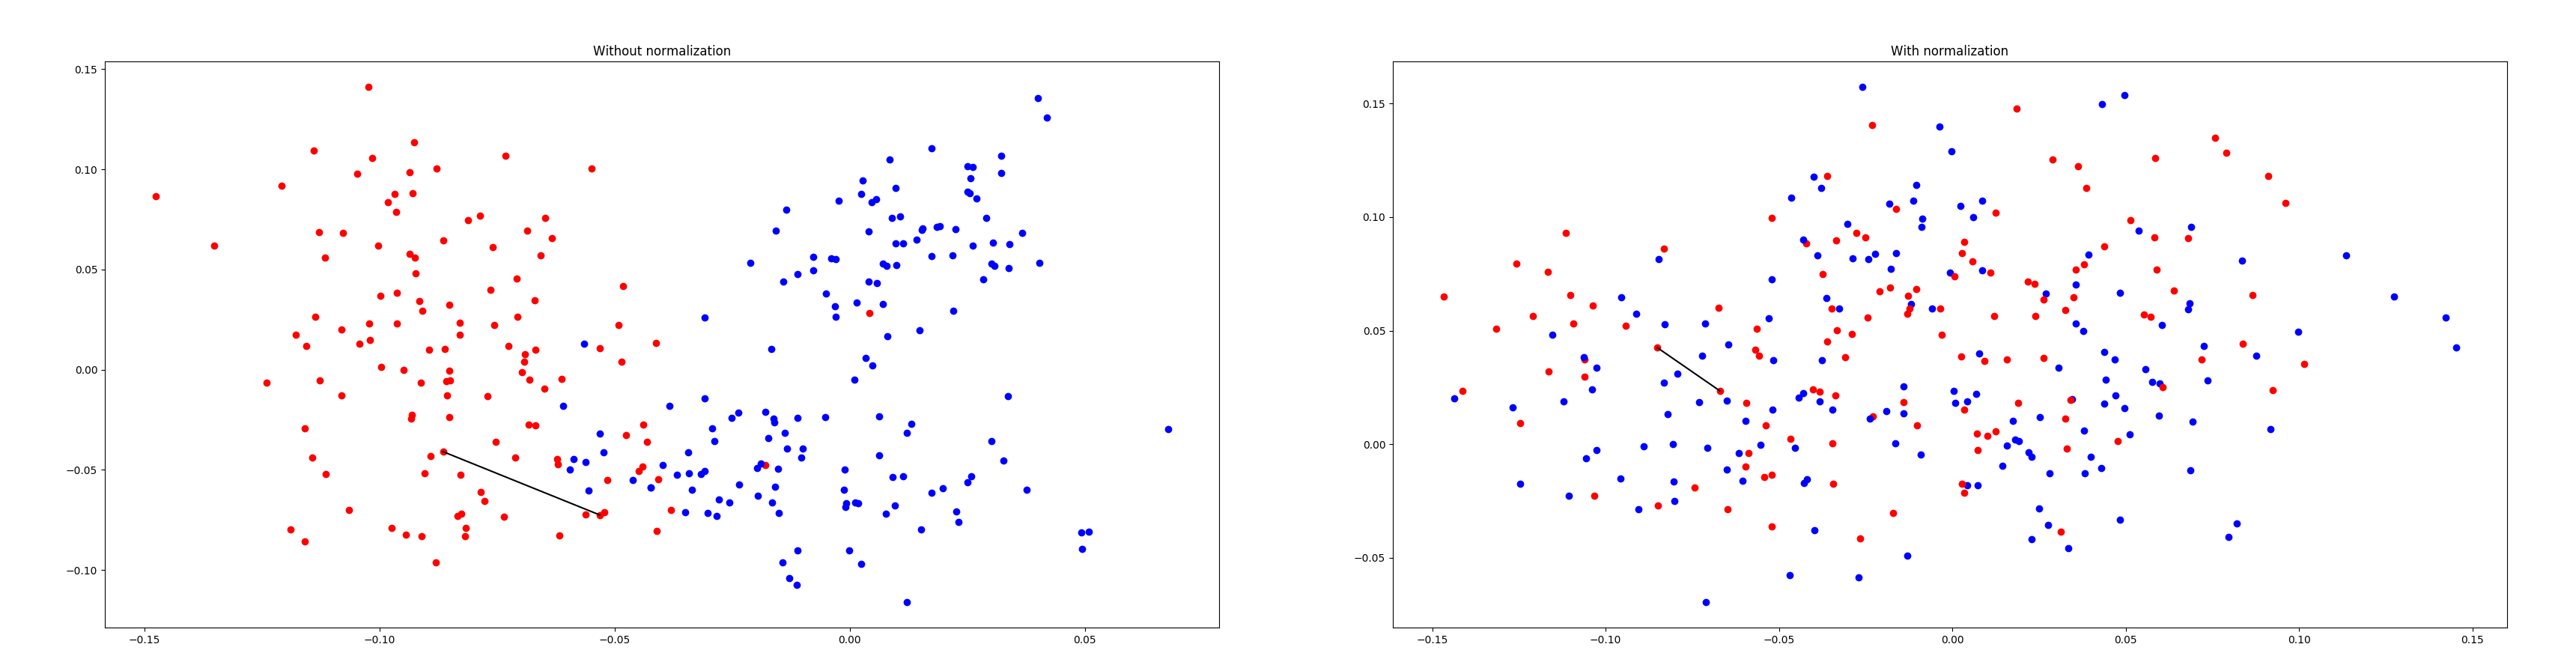
\includegraphics[width=\textwidth]{img/answers_normalization}
  \caption{Effect of filtering out users}
  \label{fig:answers_normalization}
\end{figure}

It is worth mentioning that there would be some difference between user answer performance even if users in the system do not have a preference for a single answer. But they should be distributed only close to 0.0.

We can use this to filter out users which difference in performance is too large. We thought that this would remove the separation of items based on a correct answer from a projection. Figure~\ref{fig:answers_normalization} shows projection before and after filtering out users that have a great difference in performance on items by their answer. Colors in this particular image represent correct answers to items. It is visible that separation by answer is less visible after filtering out part of the users.

In this particular case, we consider that user should be filtered out when his difference on answers is greater than 0.2. This value was chosen based on comparing our histogram with simulated data.

% answer regularity summary

To sum it up. When we simulated users, we gave them all habit to use one answer more commonly. This divided items by their corresponding correct answer. But not all users have a habit of using one answer by default in real-world data. Yet there is quite a large amount of users who do. We can filter them out to stop them affecting projections.

% > Levels regularity

\section{Levels regularity}\label{evaulation-levels-regularity}

This section describes in detail some of our experiments we concluded that relate to the formation of items into clusters of the same level. It describes two experiments showing high-level factors that can cause level regularity.

% > > Missing values

\subsection{Missing values}\label{missing-values}

% Can missing data affect the result of similarity calculation?

As we mentioned before, performance matrix is relatively sparse. However, missing values are not distributed randomly, but they form a pattern. Our question is whether this pattern of missing values can affect similarity of items and projections.

% structure of performance matrix

Items in each item-set of the system are divided into up to three levels. The difficulty of the levels differs. That is why users in the system usually do not solve all of the available levels (this is also shown in Figure~\ref{fig:missing_pattern_diagram}). Less experienced users tend to solve only first or first two levels. Still, more experienced users solve only higher levels. This is causing visible pattern in performance matrix. Some user rows contain information only about specific levels and are missing all values of other levels.

\begin{figure}
  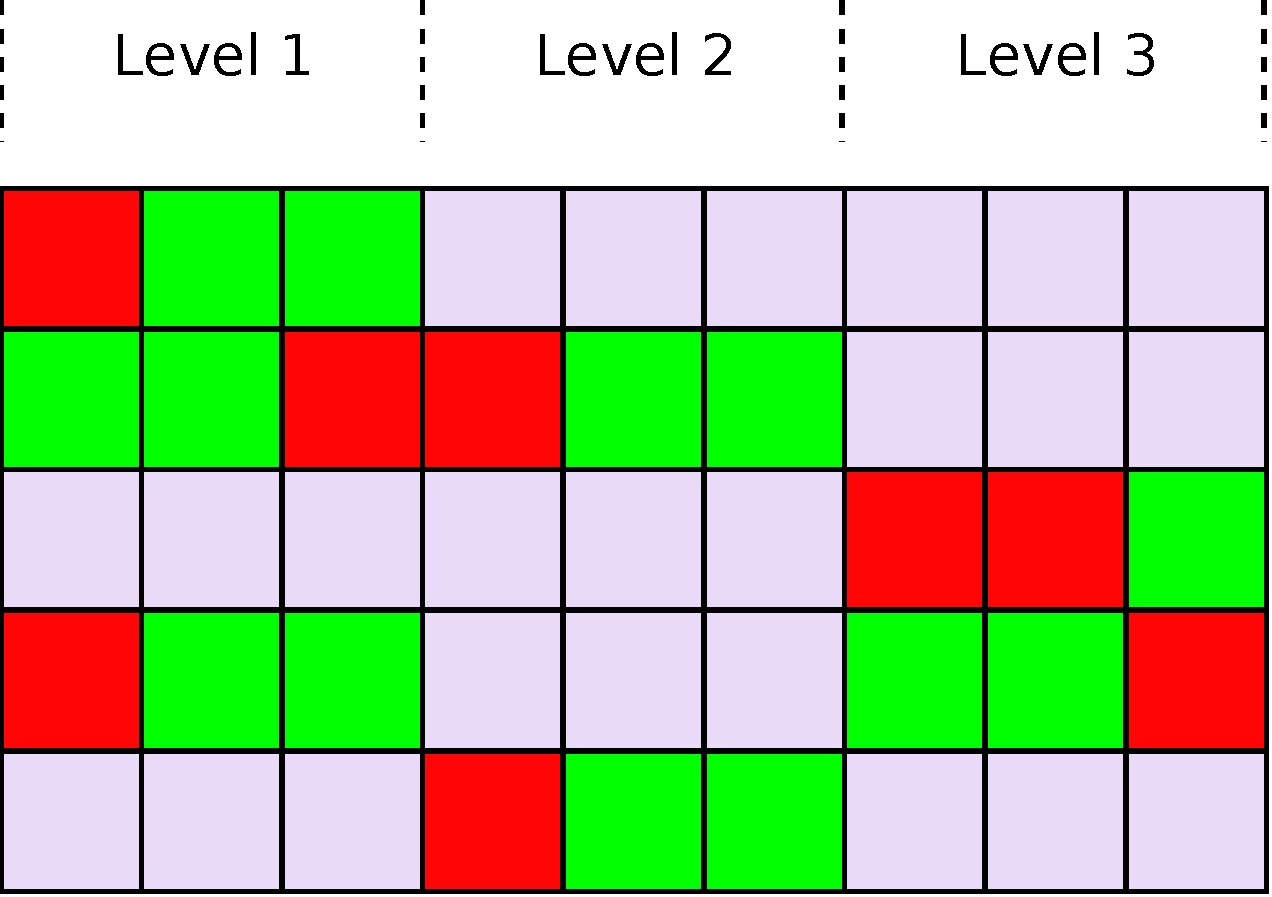
\includegraphics[width=5cm]{img/missing_pattern_diagram}
  \caption{Diagram showing pattern of missing data}
  \label{fig:missing_pattern_diagram}
\end{figure}

% > > > Simulation of missing values

\subsubsection{\textit{Simulation of missing values}}\label{simulation-of-missing-values}

Once again, we use simulation to verify whether this factor can cause such regularity. This simulation is also constructed similarly as one we explained before in section~\ref{simulated-data}. The only difference is that resulting performance matrix will now contain missing values. We achieve this by requiring simulated users to solve only some items. Each user starts with solving one level and then with some probability continues to another. So most users solve only one level, some users solve two levels, and only a few users solve all three levels. Order in which they answer levels is chosen at random as users are not required to continue chronologically.

\begin{figure}
  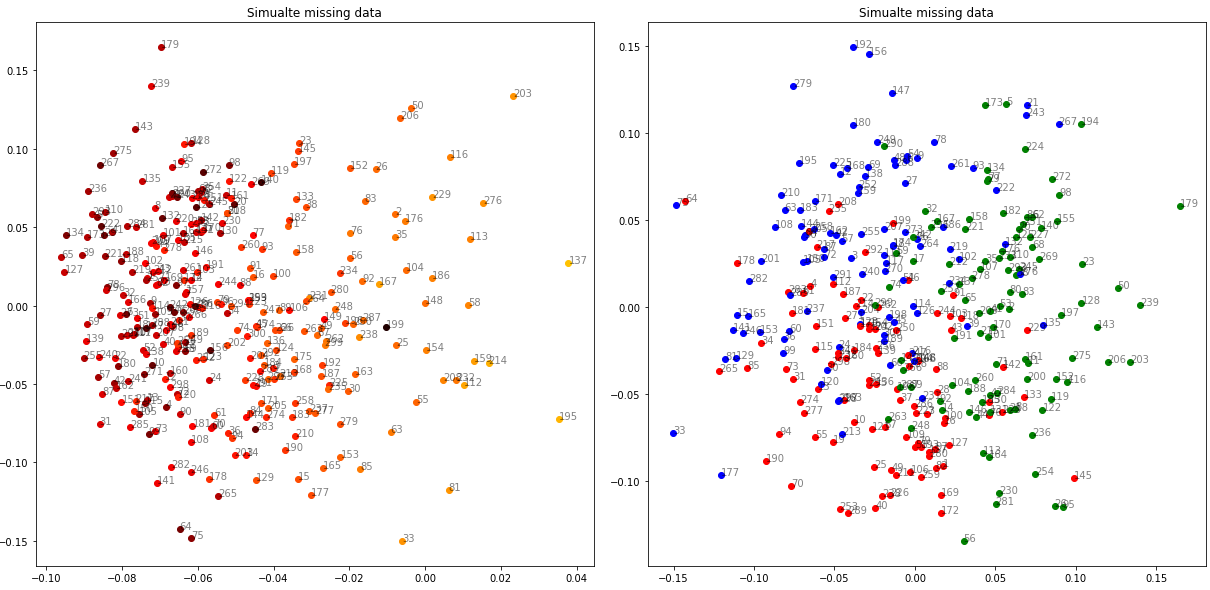
\includegraphics[width=\textwidth]{img/simulated_missing}
  \caption{First and second (left) and second and third (right) principal components of PCA on simulated data}
  \label{fig:simulated_missing}
\end{figure}

Figure~\ref{fig:simulated_missing} shows two resulting projections of simulated data with missing answers. There are two shown projections. They are both colored by a level of items. Difference between this projections is that one on the left shows first two principal components of PCA, while second projection shows second and third component of PCA. So there are three dimensions shown effectively.

In this particular projection, the first dimension corresponds pretty well with the difficulty of items and next two dimensions (second image) distinguish belongingness to each level. However, such easy explanation of axis is possible only for simulated data. When looking at projections of real data, it is much harder to describe its axis.

This simulation showed that pattern of missing data could cause clusters of items.

% > > > Cause of missing data regularity

\subsubsection{\textit{Cause of missing data regularity}}\label{cause-of-missing-data-regularity}

After looking at similarity matrix of this particular simulated data, we noticed that there is a slight difference between similarities in the same level and similarities of items in different levels. There is a visible difference in stability. Similarity values of items in different levels contain much more noise than items in the same level. This causes projection to consider items on the same level as more similar.

However, this is not true in general only if an amount of users who solved items in more than one level is small enough. If we increase the number of simulated users by ten times, we get stable similarity and no clusters. In other words, the value of similarity is not affected by the amount of data, but its stability is. And this can also appear in final use-case.

The pattern of missing data is another high-level factor that we explained and can cause regularities in item similarities.

% > > Item performance

\subsection{Item performance}\label{item-performance}

Another possible factor affecting similarities and therefore projections can be difficulty od items. The first part of this section analyzes difficulty of items in the tutoring system. Then we try to replicate this data using simulation.

\begin{figure}
  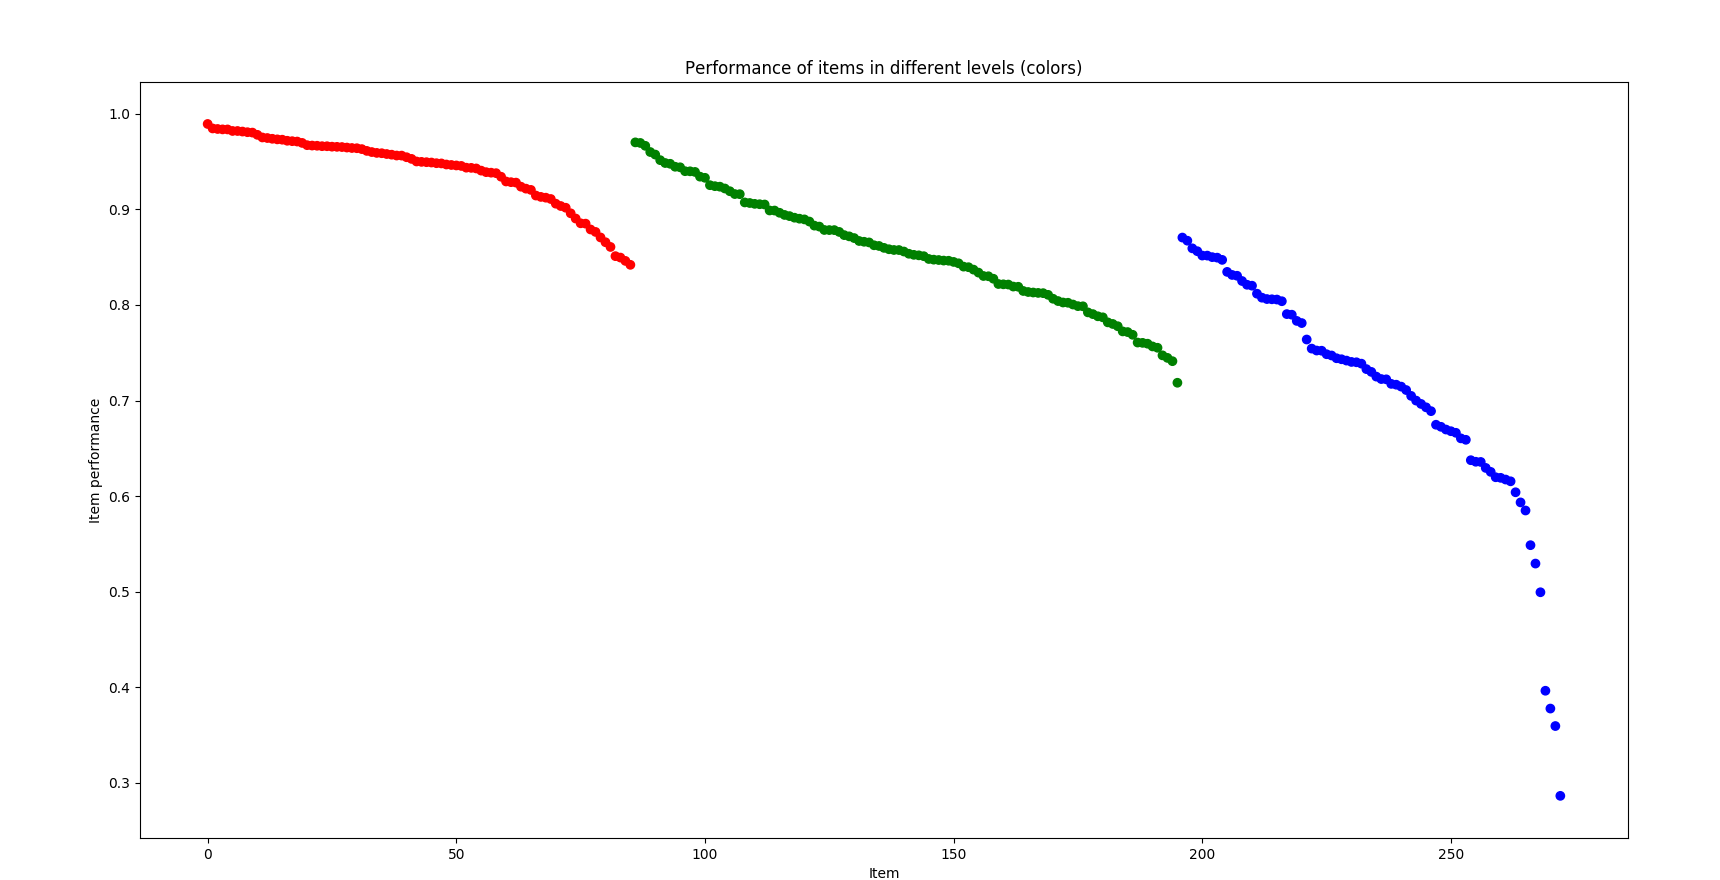
\includegraphics[width=8cm]{img/items_performance_levels}
  \caption{Boxplot showing performance of items divided into three levels}
  \label{fig:item_performance_levels}
\end{figure}


Figure~\ref{fig:item_performance_levels} shows boxplot of items performance (ratio of correct answers to all answers) from one item-set. Given item-set contains three levels with mean performances 94\%, 86\%, and 71\% respectively.

Items are divided in such manner that difficulty of levels raises. However, this division is not strict. It is visible on Figure~\ref{fig:item_performance_levels} that difficulty of items in levels overlaps. Question is whether the difficulty of items is somehow projected into similarity of items.

For this simulation, we variate difficulty of questions. In the standard simulation, we use the difficulty of items drawn from same normal distribution $\mathcal{N}(0,\,1)$. The only difference is that we alternate mean value of normal distributions for each simulated level. For this particular experiment, we fitted this shifts to correspond to performances observed in real item-set ($\mathcal{N}(1.4,\,1), \mathcal{N}(2.0,\,1), \text{and} \mathcal{N}(3.0,\,1)$).

% different performance of items in levels does not cause such clusters

Results are visible in Figure~\ref{fig:simulated_performance}. We concluded that this factor could also cause clusters of items from the same level. However, they are not as apparent as with the previous factor of pattern in missing data.

\begin{figure}
  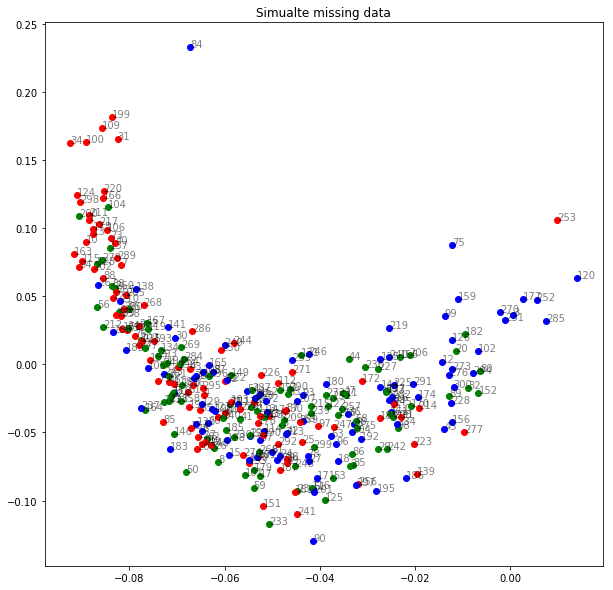
\includegraphics[width=8cm]{img/simulated_performance}
  \caption{Three simulated levels with different mean performance}
  \label{fig:simulated_performance}
\end{figure}

% --------------------------- %
% Recommendations             %
% --------------------------- %

\chapter{Recommendations}\label{recommendations}

% super intro

This short chapter summarizes recommendations gathered after looking at results of our experiments. We list both general recommendations that we think are useful for everyone and practical recommendations for future work on this specific tutoring system.

% > Factors affecting different stages

\section{Factors affecting different stages}\label{factors-affecting-different-stages}

\begin{figure}
  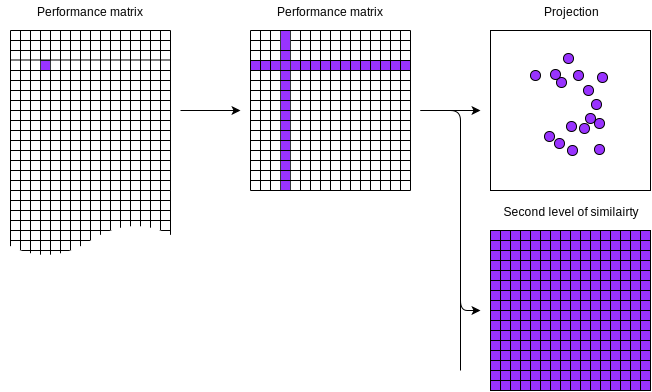
\includegraphics[width=10cm]{img/affected_diagram}
  \caption{Diagram of possibly affected values on different stages of processing}
  \label{fig:affected_diagram}
\end{figure}

% affected a portion of data on different stages of the pipeline

As we have learned, there are a few stages used in our pipeline for computing similarity. Figure~\ref{fig:affected_diagram} depicts the possible effect of single value changed in a log of users performance. Apparently, in performance matrix, this is only single value. When we continue with computing similarity matrix single row and single column can be affected in some way. On this stage, it is still straight as answers to item affect only similarities which include this item. Although, when we apply next stage of processing like projection, or clustering single changed value can affect all of the items.

% intro affected a portion of data on different stages of the pipeline

In the third chapter~\ref{evaluation} we described a few high-level factors that can cause regularities in similarity that we found. There were only three high-level factors that we tested, but we can already divide them into two categories based on how they affect similarities of items.

\begin{table}
  \setlength{\tabcolsep}{0.12em} % for the horizontal padding
  {\scriptsize\renewcommand{\arraystretch}{1.0}% for the vertical padding
    \begin{tabular}{ | l | l l l | }
      \hline
      \cellcolor[gray]{1.0} & Users preferring one answer      & Pattern in missing data & Mean level performance            \\
      \hline
      Performance           & Uneven performance for user      & Missing values          & Mean performance of items         \\
      Similarity            & Higher similarity of some answer & Stability of similarity & Higher similarity of some level   \\
      Projection            & Clusters                         & Clusters                & Clusters                          \\
      \hline
    \end{tabular}
  }
  \caption{Effect of high-level factors on different stages of similarity pipeline}
  \label{tab:effect-of-factors-on-stages}
\end{table}

Table~\ref{tab:effect-of-factors-on-stages} summarizes how described high-level factors affect each stage of similarity pipeline. When we use similarity for computation of projection in at the last stage, they all cause some clusters. However, they all differ in how they affect stages before the last stage. For example in similarity matrix, two of observed factors cause higher similarity of some group of items while the factor of pattern in missing data only affects the stability of values (affects it indirectly).

It is worth knowing how high-level factor can affect each stage of similarity pipeline. The factor of missing answers does not affect outlier detection techniques which utilize only the similarity of items. (Only if technique compares them to each other, this factor affects the result.)

% > Practical recommendations

\section{Practical recommendations}\label{practical-recommendations}

We now understand used similarity pipeline. Therefore we can give some recommendations for future work on this tutoring system.

% similarity

For developers of the system it is worth knowing that structure of user interface can affect data in some unexpected way (refer to section~\ref{regularities}). In case that similarity would be used extensively it may be useful to implement some changes to the user interface to prevent such regularities.

% data normalization

Another possible solution is to normalize data in some way when processing them. In section~\ref{user-answer-performance} we proposed one such normalization for the factor of using one answer by default. However, it is not so straightforward to normalize factor of missing answers.

% similarity measure choice

We did not find any difference in the usability of observed similarity measures. Therefore we recommend using any measure that is good performing and convenient to use. Based on previous research this can be Pearson correlation coefficient applied two times sequentially. This measure has good stability of results even on smaller datasets and is easy to implement.

% projection and clustering are affected the same

Projection and clustering both suffer from same problems. They are both affected by all described high-level factors.

% in outlier detection

For outlier detection, we can recommend using method that does not depend on the global distribution of values, only on the local neighborhood as items with some answers have higher similarity. Another possibility is to normalize data in some way. One example has proposed the removal of users with a great difference of answer preference. But other less drastic normalization methods can also be found we only used this one to show that these users are a cause for this separation of items by correct answer.

% does not matter

We also found multiple properties that do not affect anything. E.g., the ratio of correct answers in item-set does not affect similarity. Item performance does not correlate with its similarity. Also considering users first or the last answer to given item does not matter.

%HACK check, whenever modifying text
\clearpage

% > General recommendations

\section{General recommendations}\label{general-recommendations}

As we saw, when using similarity with some particular dataset problems specific to it may arise. While trying to explain this patterns in our particular data we used we run into multiple situations which can repeat even when explaining some different data using similarity techniques. That is why we also want to give some general recommendations.

% determine range

We think it is always a good idea to first determine the if behavior we are interested in is present in whole dataset and all even when we alter used techniques. We determined whether is observed behavior present in all item-sets and using any similarity measure. This experiments were explained in first section~\ref{evaluation-basic} of the previous chapter and helped us a lot in understanding regularities.

% simulations

We found it useful to use simulations when we are dealing with techniques from which we obtain some results, but it is hard to explain why (projection). Altering inputs and observing output is a way of explaining what is happening inside.

% more dimensions of PCA

Usually, when using PCA only first two principal components are used. But we found it useful to look at following dimensions as well. This approach was used in section~\ref{missing-values} when the first dimension correlated with the performance of items and did not give us any useful information. Only looking at following dimensions gave us any useful information.

% --------------------------- %
% Conclusion                  %
% --------------------------- %

\chapter{Conclusion}

% What we did, what important discoveries we found

We explored differences in using different methods for measuring the similarity of educational items based on data about the correctness of users answers. Before starting this work, we knew there were some unclear circumstances considering the formation of clusters in projection and therefore the distribution of similarities of items. All the experiments we concluded were focused on this behavior. Now we understand how the structure of system may affect performance data and similarity of items itself.

We determined whether this behavior is present in whole dataset and all similarity measures or not. Multiple experiments using both real and simulated data were concluded. And as a result, we were able to answer questions proposed in section~\ref{specific-questions}. We found multiple high-level factors that can cause regularities that were validated using simulations. We explained three high-level factors that can be cause for observed regularities in similarity. We showed that in real data there might be multiple factors causing level regularity.

Most of the findings discovered in this dataset may not be directly transferable to another tutoring system. But used analysis can also help understand other tutoring systems.

% wider view of the solved problem, robomise

Adaptive learning group currently focuses on tutoring systems for teaching introductory programming. This research may also benefit from some of our findings. Before beginning work on this thesis, I also contributed to research about the similarity of programming problems~\cite{pelanek2018programming}.

Alternatively, some of the results may be even transferable into a system that is not used for learning but contains items with similar properties.

% Ideas for future work

This work was concluded as exploration analysis, and hence its results consist mostly of gathered information and recommendations for future work. In particular, implementing proposed recommendations when using similarity of items in mentioned tutoring system. The similarity of items is currently not used in the system \umimeCesky{} but increasing number of items will soon call for some automated management of problem pool. For this reason, it will be useful to analyze methods for detecting problems with item pool further.

In particular, compare the usefulness of different visualizations for authors making decision about system. Also, implementation of automatic detection of duplicate and outlier items may be useful. In some special cases, it may be even possible to recommend kinds of items that are missing from the system using similarity of items.

It also may be useful to look at the same data from another perspective and observe whether there are similar regularities when we calculate similarities of users instead.

% Recapitulation of how well we finished our task

However, we already fulfilled our goals for this work and answered questions we asked.

% See ya

\makeatletter\thesis@blocks@clear\makeatother
%\phantomsection %% Print the index and insert it into the
%\addcontentsline{toc}{chapter}{\indexname} %% table of contents.
%\printindex

\appendix %% Start the appendices.

% > Attached files

\chapter{Attached files}

Concluded experiments are collected in Jupyter notebooks which also use scripts written in Python to simplify our work and make notebooks cleaner. There are also some additional experiments not described in this text as we chose to include here only experiments with somehow surprising results or experiments that gave us the most insight into problems we were solving. Providing all the experiments in this way gives everyone possibility to alter and re-execute them. More information about launching this environment is present in enclosed files.

However, the used dataset is not publicly available therefore enclosed data are obfuscated. Item statements were replaced with randomly generated strings.

List of most important files:

\begin{itemize}[\null]
\item \texttt{components/} - Python scripts used to make our work cleaner
\item \texttt{data/} - Dataset used for analysis
\item \texttt{docs/} - Further describes how to use this environment
\item \texttt{notebooks/} - Contains four notebooks with analysis
\item \texttt{README.md} - Detailed instructions on how to start the environment
\end{itemize}

\end{document}
